\documentclass{llncs}
\newcommand{\Section}[1]{\vspace{-8pt}\section{\hskip-1em.~~#1}\vspace{-3pt}}
\newcommand{\SubSection}[1]{\vspace{-3pt}\subsection{\hskip -1em.~~#1}\vspace{-3pt}}

% \section{mathematical notation}
\usepackage{hyperref,color}
\newcommand{\vect}[1]{\mathbf{#1}}
\newcommand{\field}[1]{\mathbf{#1}}
\newcommand{\image}[1]{#1}
\newcommand{\I}{\image{I}}
\newcommand{\J}{\image{J}}
\renewcommand{\u}{\vect{u}}
\renewcommand{\v}{\vect{v}}
\renewcommand{\c}{\vect{c}}
\newcommand{\h}{\vect{h}}
\newcommand{\w}{\vect{w}}
\newcommand{\myphi}{\phi}
\newcommand{\mypsi}{\psi}
\newcommand{\D}{D}
\renewcommand{\d}{\nabla}
\newcommand{\dd}{\text{d}}
\newcommand{\p}{\partial}
\renewcommand{\L}{\Delta} % laplacian
\newcommand{\R}{\mathbb{R}}
\newcommand{\myS}{S}
\newcommand{\myR}{R}
\newcommand{\myE}{E}
\newcommand{\ld}{\langle}
\newcommand{\rd}{\rangle}
\newcommand{\LL}{\mathcal{L}} % operator L
\newcommand{\tQ}{\mathcal{Q}}
\newcommand{\Id}{\text{Id}}
\newcommand{\tG}{{G}} % operator L
\newcommand{\Diff}{\text{Diff}}
\newcommand{\VV}{\mathcal{V}}
\newcommand{\opL}{\mathcal{L}}

\newcommand{\X}{{\bf X}}
\newcommand{\x}{{\bf x}}
\newcommand{\Y}{{\bf Y}}
\newcommand{\y}{{\bf y}}
\newcommand{\Z}{{\bf Z}}
\newcommand{\z}{{\bf z}}
\newcommand{\bs}{\boldsymbol}
\newcommand{\bSigma}{\boldsymbol \Sigma}
\newcommand{\bsp}{$\substack{
   \rightsquigarrow \\
   b
  }$}
\newcommand{\mi}{$\substack{
   \approx \\
   \text{mi}
  }$}
\newcommand{\cc}{$\substack{
   \approx \\
   \text{cc}
  }$}
\newcommand{\tk}{~ITK$^{\text{4}}$~}
\usepackage{amsmath,amssymb,algorithm,algorithmic}
\usepackage{times}
\usepackage{setspace,verbatim}
\usepackage{epsfig}

\begin{document}
\vspace{-0.1in}
\title{A unified image registration framework for ITK}
\author{Brian B. Avants, Nicholas J. Tustison$^\dagger$, Gang Song,\\ Baohua Wu,
  Michael Stauffer, James C. Gee}
\institute{Penn Image Computing and Science Lab \\ Dept. of Radiology \\University of
  Pennsylvania, Philadelphia, PA, 19104\\ 
  $^\dagger$Dept. of Radiology, \\ University of Virginia,
  Charlottesville, VA 22903}
\maketitle              
\begin{abstract}
Publicly available scientific resources help establish evaluation
standards, provide a platform for teaching and may improve reproducibility.
Version 4 of the Insight ToolKit (\tk) seeks to establish new
standards in publicly available image registration methodology.  In this
work, we provide an overview and preliminary evaluation of the revised
toolkit against registration based on the previous major ITK version
(3.20).  Furthermore, we propose a nomenclature that may be used to
discuss registration frameworks via schematic representations.  In
total, the \tk contribution is intended as a structure to support
reproducible research practices, will provide a more extensive
foundation against which to evaluate new work in image registration
and also enable application level programmers a broad suite of tools
on which to build.
\end{abstract}

\section{Introduction}
As image registration methods mature---and their capabilities become
more widely recognized---the number of applications increase
\cite{Rueckert1999,2004,Shelton2005,Miller2005,Chen2008,Cheung2009,Baloch2009,Peyrat2010,Metz2011,Kikinis2011,Fedorov2011,Murphy2011}.
Consequently, image registration transitioned from being a field of active research, and few applied results, to a
field where the main focus is translational.  Image registration is
now used to derive quantitative biomarkers from images
\cite{Jack2010a}, plays a major role in business models and clinical
products (especially in radiation oncology) \cite{Cheung2009}, has led
to numerous new findings in studies of brain and behavior (e.g. \cite{Bearden2007}) and is a critical component in applications in
pathology, microscopy, surgical planning and more
\cite{Shelton2005,Miller2005,Floca2007,Chen2008,Cheung2009,Peyrat2010,Kikinis2011,Murphy2011}.
Despite the increasing relevance of image registration across
application domains, there are relatively few reference algorithm
implementations available to the community.

% \cite{Jenkinson2001,Christensen1996,Rueckert1999,Yoo2002,Ackerman2003,2004,Shelton2005,Wolf2005,Miller2005,Floca2007,Chen2008,Khan2008,Cheung2009,Vercauteren2009,Baloch2009,Klein2010,Peyrat2010,Taka2011,Metz2011,Kikinis2011,Fedorov2011,Murphy2011,Avants2011}.

% itk 

% ideas 

% Taka2011,Metz2011,,Fedorov2011,,}.
% {\bf How is image registration applied?}

% {\bf What role has ITK filled in the registration world?}  

One source of benchmark methodology is the Insight ToolKit (ITK)
\cite{Yoo2002,Ackerman2003}, which marked a significant contribution to
medical image processing when it first emerged over 10 years ago.
Since that time, ITK has become a standard-bearer for image
processing algorithms and, in particular, for image registration
methods.  In a review of ITK user interests, image registration was cited as the most important
contribution of ITK (personal communication).  Numerous papers use ITK
algorithms as standard references for implementations of Demons
registration and mutual information-based affine or B-Spline
registration \cite{2004,Shelton2005,Floca2007,Chen2008,Cheung2009}.
Multiple toolkits extend ITK registration methods in unique ways.
Elastix provides very fast and accurate B-Spline registration
\cite{Klein2010,Murphy2011}.  The diffeomorphic demons is a fast/efficient
approximation to a diffeomorphic mapping \cite{Vercauteren2009}.  
ANTs provides both flexibility and high average performance
\cite{Avants2011}.  The BrainsFit algorithm is integrated into slicer
for user-guided registration \cite{Kikinis2011}.
Each of these toolkits has both strengths and weaknesses
\cite{Klein2010,Murphy2011} and was enabled by an ITK core.    
%  What papers use ITK as a standard for comparison?  What other software builds on ITK registration?

%How does the v4 registration framework build on the past?  What does it contribute that's new?  
% What is it? Why were these the tools we chose to contribute?  
% {\bf \tk Registration: What it is.}
The Insight ToolKit began a major refactoring effort in 2010.
The refactoring aimed to both simplify and extend the techniques available in version
3.x with methods and ideas from a new set of prior work
\cite{Jenkinson2001,Christensen1996,Rueckert1999,Miller2005,Peyrat2010,Avants2011}.
To make this technology more accessible, \tk unifies the dense
registration framework (displacement field, diffeomorphisms)
with the low-dimensional (B-Spline, Affine, rigid) framework by
introducing composite transforms, deformation field transforms and
specializations that allowed these to be optimized efficiently.  A sub-goal set for \tk was to simplify
parameter setting by adding helper methods that use well-known
principles of image registration to automatically scale transform
components and set optimization parameters.  \tk transforms are also
newly applicable to objects such as vectors and tensors and will take into account covariant geometry if
necessary.  Finally, \tk reconfigures the registration framework
to use multi-threading in as many locations as possible.
The revised registration framework within ITK is more thoroughly
integrated across transform models, is thread-safe and provides
broader functionality than in prior releases. 

% graceful failure of an algorithm.  Should not be catastrophic. A nice feedback loop for software.  

%{\bf procedure: 1. clinicians are conservative.  2.  first, prove robustness.  3. provide useful and encouraging feedback.  4. fail gracefully when do fail.   }

% good average performance versus good performance on a given dataset.

The remainder of the document will provide an overview of the new
framework via the context of a potential general nomenclature.  We
also establish performance benchmarks for the current \tk
registration.  Finally, we discuss future developments in the
framework.

\section{Nomenclature}
The nomenclature below designates an image registration
algorithm pictorially.  This nomenclature is intended to be a
descriptive, but also technically consistent, system for visually
representing algorithms and applications of registration.  Ideally,
any standard algorithm can be written in the nomenclature below.
\begin{description}
\item [A physical point:] $x \in \Omega$ where $\Omega$ is the domain,
  usually of an image.
\item [An image:]  $ I \colon \Omega^d \to \mathbb{R}^n$ where $n$ is the
  number of components per pixel and $d$ is dimensionality.  A second
  image is $J$. 
\item [Domain map:] $ \phi \colon \Omega_I \to \Omega_J $ where $\to$ may be
  replaced with any mapping symbol below. 
\item [Affine mapping:] $\leftrightarrow$ a low-dimensional invertible 
  transformation: affine, rigid, translation, etc. 
\item [Affine mapping:] $\rightarrow$ designates the direction an
  affine mapping is applied.  
\item [Deformation field:] $ \rightsquigarrow$ deformation field mapping $J$
  to $I$.  May not be invertible.
\item [Spline-based mapping:] $\substack{
   \rightsquigarrow \\
   b
  }$ e.g. B-Spline field mapping $J$
  to $I$.
\item [Diffeomorphic mapping:] $ \leftrightsquigarrow$ these maps
  should have an accurate inverse that is computed in the algorithm or can be computed from the results.
\item [Composite mapping:] $\phi=\phi_1(\phi_2(x))$ is defined by
  $ \leftrightsquigarrow \rightarrow $ where $\phi_2$ is of type
  $\leftrightsquigarrow$. 
\item[Not invertible:]  $\nleftrightarrow$ indicates a mapping that is
  not invertible.
\item [Similarity measure:] $\substack{
   \approx \\
   s
  }$ or $\approx_s$ indicates the metric $s$ that compares images.
% \item [Transport versus diffeomorphism] intrasubject versus intersubject.
% \item [Resolution effects]  ...
% \item [accuracy vs precision] obsessed with accuracy because we dont
% know the precision we need
% \item [Evaluation data] is there any?
% \item [Serial vs longitudinal]  short time scale versus long time scale
% \item [Pathology] appearance changes ...
% \item [whole body atlas] map any image to whole body
% \item [radiation oncology] techs understand translation versus rotation versus deformation.
\end{description}
We would then write a standard Demons registration application that maps 
one image, $J$, into the space of $I$ (presumably a template) as:
$$
 I  \rightsquigarrow \rightarrow  J \text{~~~~~which symbolizes~~~~~} I \approx
 J( A( \phi( x ) )),
$$
with $A$ an affine mapping and $\phi$ a generic deformation. 
The notation means that the algorithm first optimizes an affine
mapping, $ \rightarrow$, 
between $J$ and $I$.  This is followed by a deformation.  
The second stage computes a deformation, $\rightsquigarrow$, from $\rightarrow J$
to $I$.  In terms of transformation composition, we would write
$\rightsquigarrow \rightarrow  J = J_w(x) =
J( \phi_\text{Affine} ( \phi_\text{Demons} ( x) )) $ where $J_w$ is
the result of warping $J$ to $I$.  The $\phi$ are the specific
functions corresponding to the schematic arrows.  Note, also, that the
tail of the arrow indicates the transform's domain.  The arrowhead
indicates its range.  Finally, we denote the similarity metric as
$\approx$ which indicates a sum of squared differences (the default
similarity metric).  \tk supports metrics such as mutual information,
$\substack{ \approx \\ \text{mi} }$, or cross-correlation, $\substack{
\approx \\ \text{cc} }$.  We will use this nomenclature to write
schematics for registration applications in the following sections.

\section{Overview of the unified framework}
The key ideas for \tk registration are:
\begin{figure}[t]
\begin{center}
\begin{tabular}{c}
% 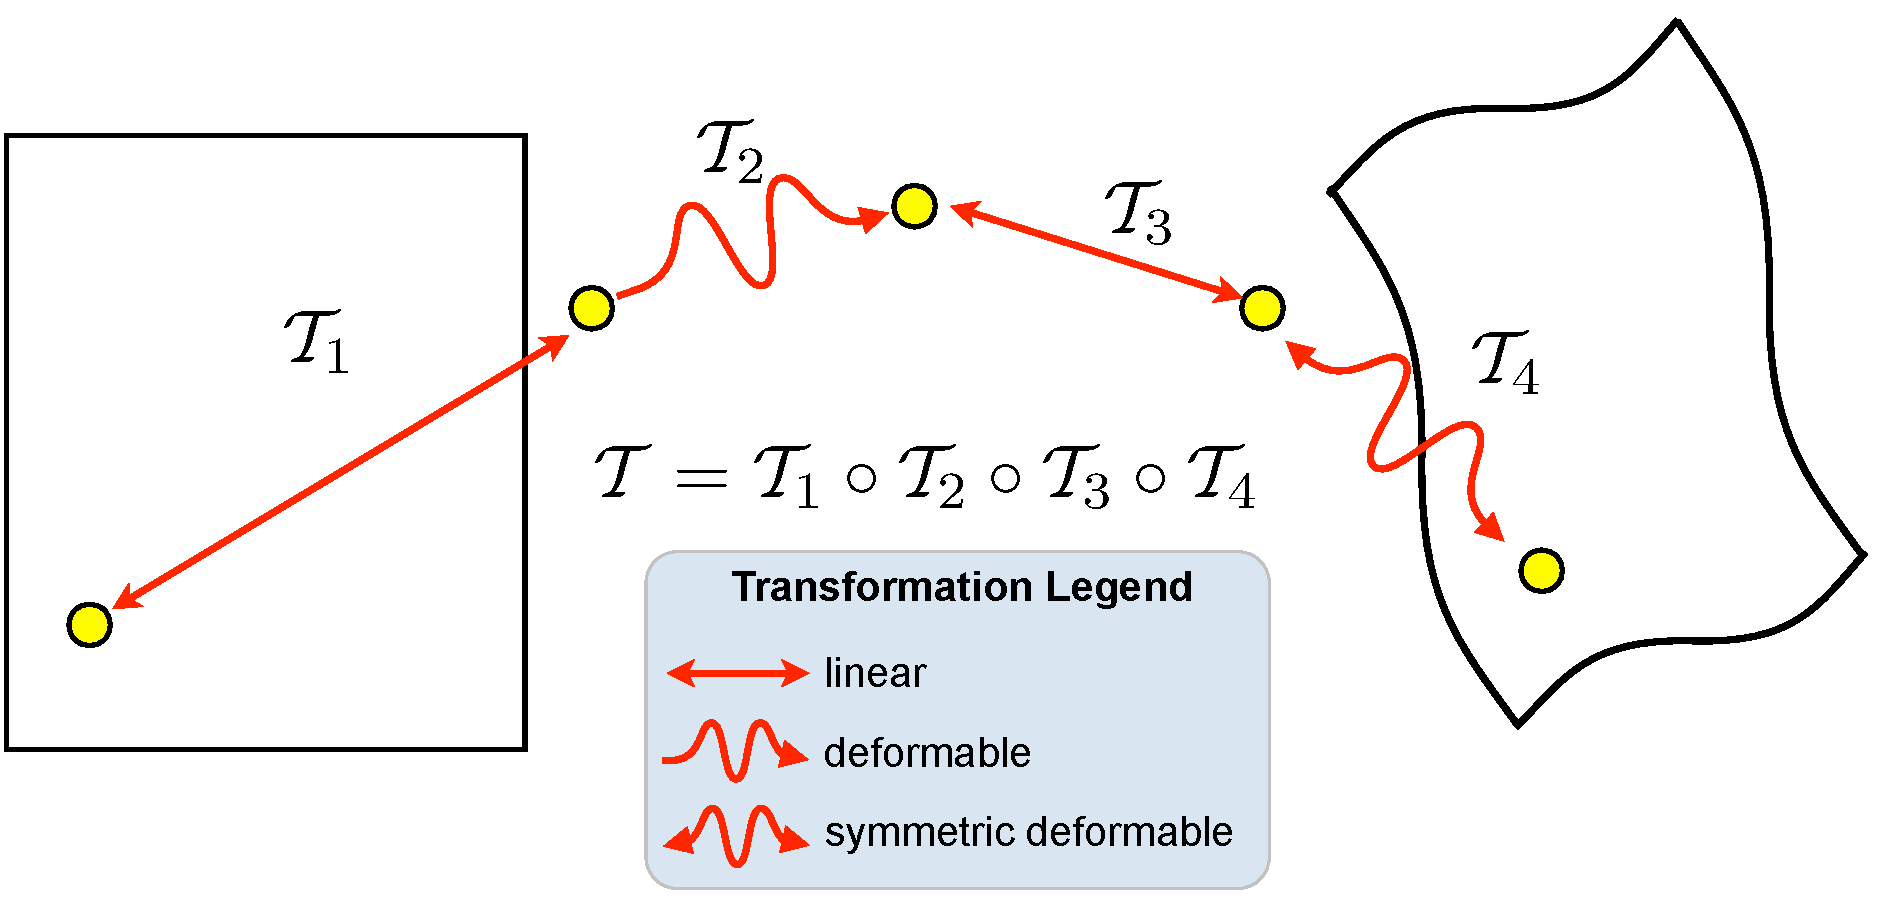
\includegraphics[width=4.5in]{figs/composemap.pdf}
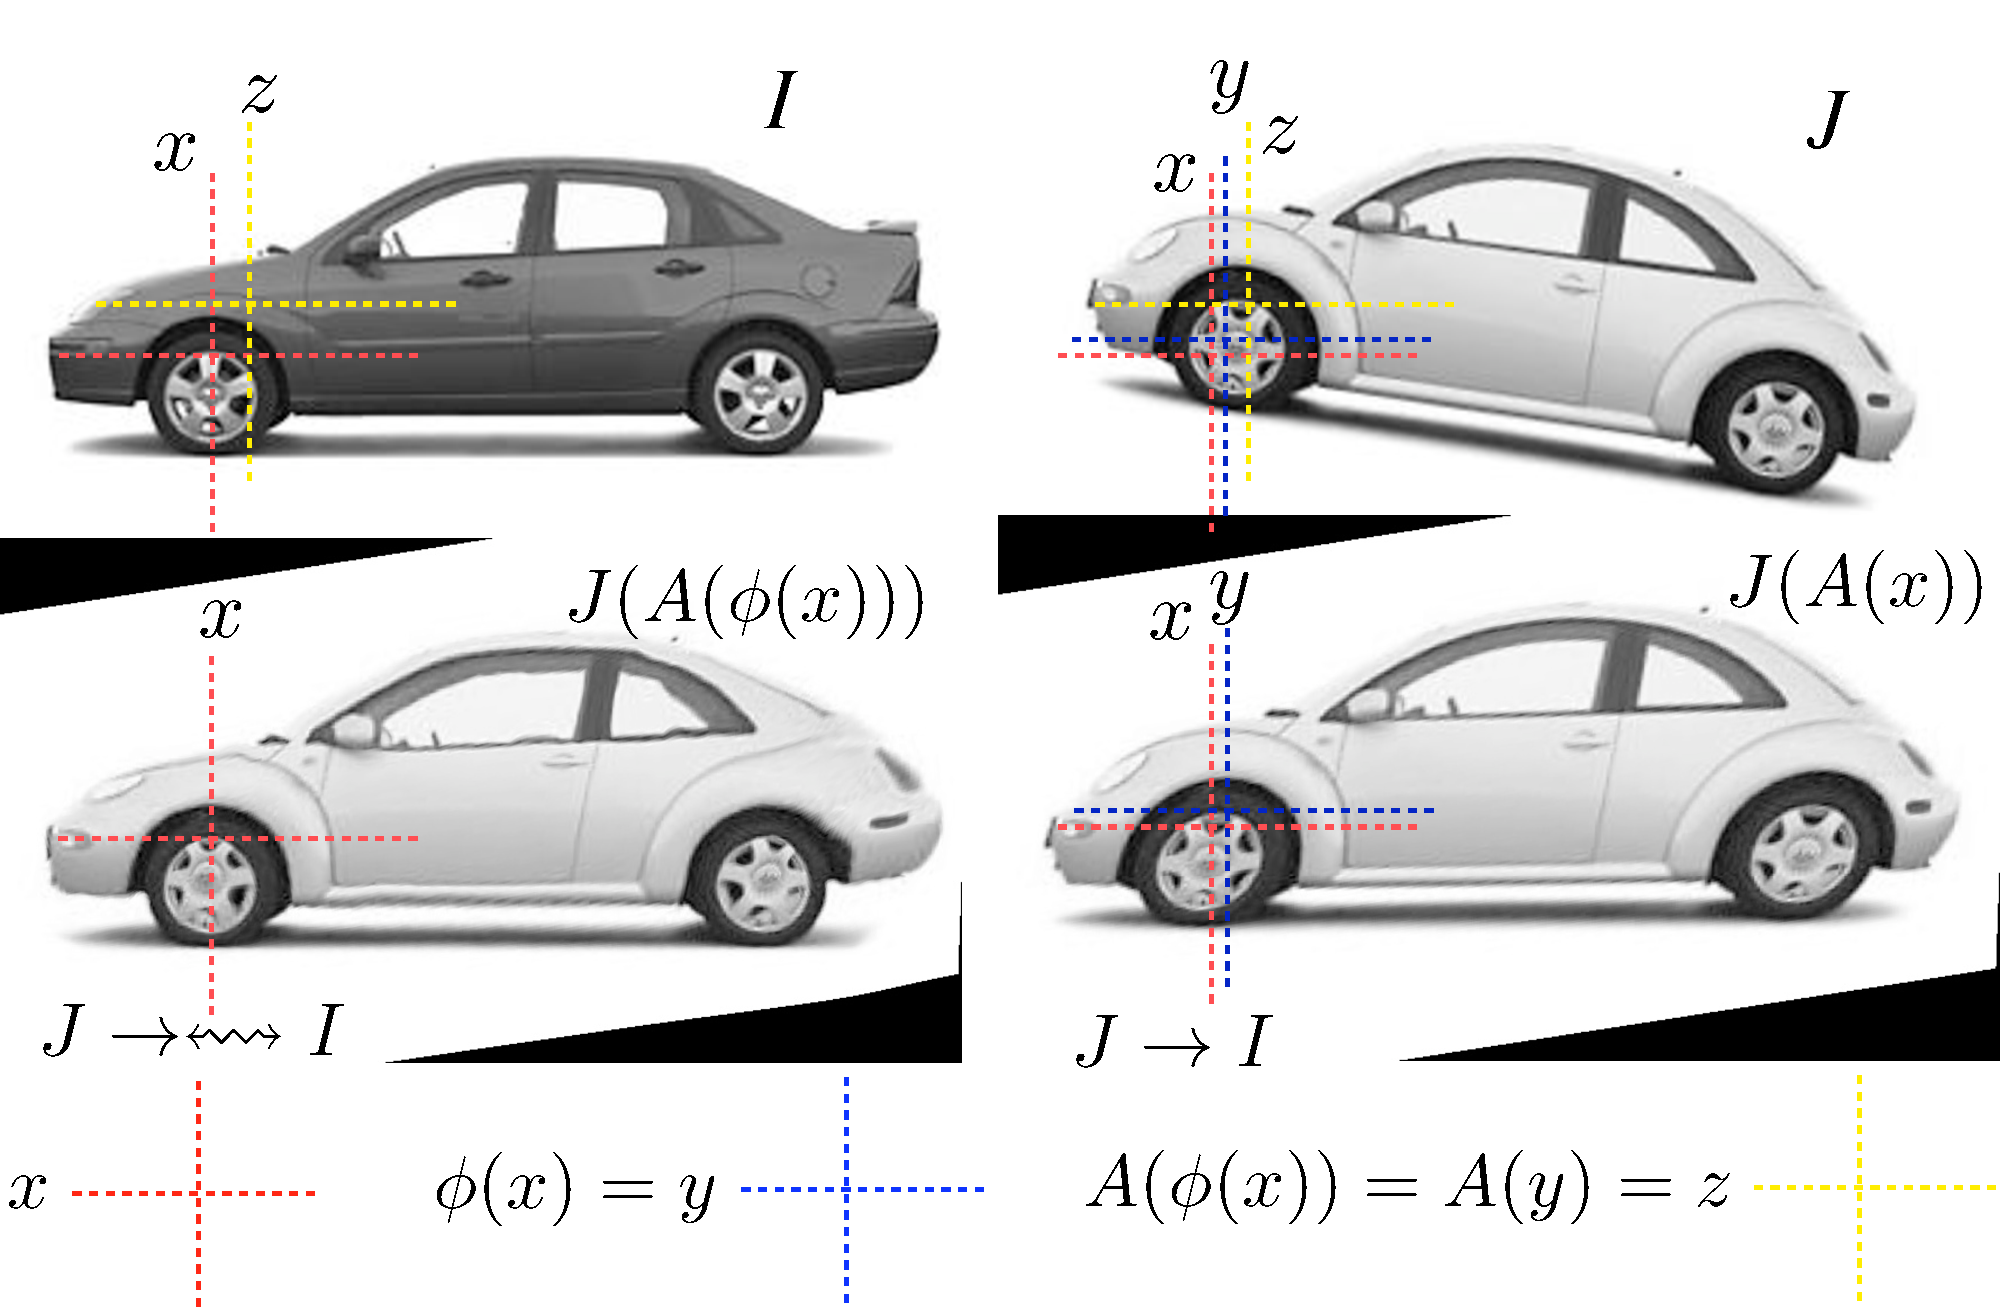
\includegraphics[width=4.5in]{figs/RegistrationNomenclature.pdf}
\end{tabular}
\caption{\baselineskip 12pt \small Define $x$ in $\Omega_I$ and $z$ in
  $\Omega_J$ as the same material point but existing in different
  domains.  The point $y$ is in a domain that is intermediate between
  $\Omega_I$ and $\Omega_J$.  The standard approach in the ITKv4
  registration framework is to map image $J$ (b) to image $I$ (a) by first
  identifying the linear transformation, $\rightarrow$, between the images, shown in (c).  Second, we remove the shape (diffeomorphic)
  differences (d).  Consequently, we have a composite mapping, computed via the
  mutual information similarity metric, that identifies
  $I(x) ~\approx_\text{mi}  J(A(\phi(x))) =  J_\text{Affine}(y) = J(z)
  $. The image $J_\text{Affine}(y)$
  represents $J$ after application of the affine transformation $A$
  i.e. $J(A(x))$.}
%  We avoid compounding interpolation  error by concatenating transformations.  Thus, we never need to use more than  a single interpolation into the data regardless of the nature of the  sub-transforms within the composite mapping.  Because transformations may  either perform mapping or resampling, this framework also  provides the ability to handle changes in resolution.}
\label{fig:composite}
\end{center}
\end{figure}
\begin{enumerate}
\item Registration maps can be applied or optimized through the {\em
    itkCompositeTransform} which chains transforms together as in Figure~\ref{fig:composite}.
\item Each ITK$^4$ transform has either global support (affine
  transform) or local (or compact) support (a displacement field transform).   If
  any map in a composite transform has global support then the
  composite transform has global support. 
\item \tk metrics are applicable to both types of transforms and may
  optimize over dense or sparse samples from $\Omega$.  Metrics may be
  multi-channel (e.g. for registering RGB or tensor images).
\item The optimization framework is multi-threaded and memory
  efficient to allow high-dimensional transformations to be optimized
  quickly on multi-core systems.
\item The \tk optimization framework comes with parameter setting tools
  that automatically select parameter scales and learning rates for
  gradient-based optimization schemes.  These parameter setting tools
  use physical units to help provide the user with intuition on the
  meaning of parameters.  
\end{enumerate}
Below we will discuss (1) gradient-based optimization within the
framework, (2) techniques to estimate optimization parameters for
arbitrary metric and transformation combinations and (3) a generalized
diffeomorphic matching approach.  

\subsection{Optimization Framework}
The general \tk optimization criterion is summarized as:
\begin{eqnarray}
\text{Find mapping}~\phi(x,p) \in \mathcal{T}
\text{such that}~M(I,J,\phi(x,p))~\text{is minimized}. 
\label{eq:gen}
\end{eqnarray}
While, for functional mappings, this formulation is not strictly correct, the
practical implementation of even high-dimensional continuous
transformations involves parameterization. 
The space $\mathcal{T}$ restricts the possible transformations over
which to optimize the mapping $\phi$.  The arguments to $\phi$ are its
parameters, $p$, and the spatial position, $x$.  Note that, in \tk,
the image $I$ may also contain a mapping, although it is not directly
optimized in most cases.  As will be seen later in the document, this
mapping may also be used within large deformation metrics. 

The similarity metric, $M$, is perhaps the most critical component in image registration.  
Denote a parameter set as $p = (p_1, p_2 \ldots p_n)$.  
The metric (or comparison function between images) is then defined by $M(I,J,\phi(x,p))$.  For instance, $M=\|
I(x)-J(\phi(x,p)) \|^2$ i.e. the sum of squared differences (SSD) metric. Its gradient with respect to parameter $p_i$
is (using the chain rule), 
\begin{eqnarray}
 M_{p_i}=\frac{\partial M}{\partial
  p_i}=\frac{\partial M}{\partial J}\frac{\partial
  J(\phi(x,p))}{\partial \phi} \frac{\partial \phi}{\partial p_i}^T|_x
~~.
\label{eq:grad}
\end{eqnarray}
This equation provides the metric gradient specified for
sum of squared differences (at point $x$) but similar forms arise for the correlation
and mutual information \cite{hermosillo}.  Both are implemented in
\tk for transformations with local and global support.  The
$\frac{\partial J(\phi(x,p))}{\partial \phi}$ term is the gradient of $J$ at $\phi(x)$
and $\frac{\partial \phi}{\partial p_i}$ is the Jacobian of the transformation taken
with respect to its parameter.   The transform $\phi(x,p)$ may be
an affine map i.e. $\phi(x,p)=A x + t$ where $A$ is a matrix and
$t$ a translation.  Alternatively, it may be a displacement field
where $\phi(x,p)=x+u(x)$ and
$u$ is a vector field.  In \tk, both types of maps are interchangeable
and may be used in a composite transform to compute registrations that
map to a template via a schematic such as $ I \approx \rightarrow J $, $ I $ ~\mi~\bsp~$
\rightarrow  J $, $ I $~\cc~$ \leftrightsquigarrow \rightarrow J $
or, mixing similarity metrics, $I
~\approx_\text{cc}  \leftrightsquigarrow \approx_\text{mi}  \rightarrow
J_i $.  

The most commonly used optimization algorithm for image registration
is gradient descent, or some variant.   In the above framework, the
gradient descent takes on the form of
$$
\phi(p_\text{new},x)=\phi(p_\text{old}+\lambda~[ \frac{\partial
  M}{\partial p_1} , \cdots , \frac{\partial
  M}{\partial p_n} ] ,  x ),
$$
where $\lambda$ is the overall learning rate and the brackets hold the
vector of parameter updates.  Note that, as in previous versions of
ITK, a naive application of gradient descent will not produce a smooth
change of parameters for transformations with mixed parameter types.
For instance, a change $\Delta$ to parameter $p_i$ will produce a
different magnitude of impact on $\phi$ if $p_i$ is a translation rather than a
rotation.  Thus, we develop an estimation framework that sets
``parameter scales'' (in ITK parlance) which, essentially, customize
the learning rate for each parameter.  The update to
$\phi$ via its gradient may also include other steps (such as Gaussian
smoothing) that project the updated transform back to space
$\mathcal{T}$.  Multi-threading is achieved in the gradient computation, transformation update
step and (if used) the regularization by dividing the parameter set
into computational units that correspond to contiguous sub-regions of the image domain.

\begin{comment}{
In terms of code, $\frac{d\phi}{dp}|_x$ corresponds to {\em
ComputeJacobianWithRespectToParameters( mappedFixedPoint, Jacobian);
}.  Note that it is evaluated at point $x$ not at point $\phi(x,p)$.  We
then use {\em
ComputeMovingImageGradientAtPoint( mappedMovingPoint,
mappedMovingImageGradient );} to compute the moving image gradient
when there is no pre-warping.  {\em ComputeMovingImageGradientAtPoint} uses central
differences (or a gradient filter) in the moving image space to
compute the image gradient, $\frac{dJ(\phi(x,p))}{d\phi}$.

 If one is doing pre-warping, then we have an index access to the
 warped moving image.  We compute the warped $J$ as
 $J_w(x)=J(\phi(x,p))$.  Then,
\begin{eqnarray}
\frac{dJ_w}{dx}=\frac{dJ(\phi(x,p))}{d\phi}\frac{d(\phi(x,p))}{dx} \\ \notag
\frac{dJ(\phi(x,p))}{d\phi}=\frac{dJ_w}{dx}{\frac{d(\phi(x,p))}{dx}}^{-1} 
\end{eqnarray}
In code, we use {\em ComputeMovingImageGradientAtIndex( index,
mappedMovingImageGradient );} to get $\frac{dJ_w}{dx}$ and transform
this image gradient via the inverse Jacobian by calling 
{\em mappedMovingImageGradient=
TransformCovariantVector(mappedMovingImageGradient, mappedMovingPoint ); }
}\end{comment}


\subsection{Parameter scale estimation}
We choose to estimate parameter scales by analyzing the result of a
small parameter update on the change in the magnitude of physical space deformation
induced by the transformation.  The impact from a unit change of
parameter $p_i$ may be defined in multiple ways, such as the maximum shift of
voxels or the average norm of transform Jacobians \cite{Jenkinson2001}.

Denote the unscaled gradient descent update to $p$ as $\vartriangle
p$.  The goal is to rescale $\vartriangle p$ to $q = s \cdot \vartriangle p$, where $s$ is a diagonal
matrix $\text{diag} (s_1, s_2 \ldots s_n)$, such that a unit change of $q_i$ will have
the same impact on deformation for each parameter $i = 1... n$.   
As an example, we want $ \| \phi(x,p_{\text{new}}) -
\phi(x,p_\text{old}) \| = constant $ regardless of which of the
$i$ parameters is updated by the unit change.  The unit is an epsilon
value, e.g. 1.e-3.

Rewrite $[ \frac{\partial
  M}{\partial p_1} , \cdots , \frac{\partial
  M}{\partial p_n} 
 ]$ as $\frac{\partial M}{\partial J}\frac{\partial
  J(\phi(x,p))}{\partial \phi} [ \frac{\partial \phi}{\partial p_1} , \cdots , \frac{\partial \phi}{\partial p_n} ]$.
To determine the relative scale effects of each parameter, $p_i$, we
can factor out the constant terms on the outside of the bracket.  
Then the modified gradient descent step becomes
$\text{diag}(s)\frac{\partial \phi}{\partial p}$.  We identify the values
of $\text{diag}(s)$ by explicitly computing the values of $\| \phi(x,p_{\text{new}}) -
\phi(x,p_\text{old}) \| $ with respect to an $\epsilon$ change.  A critical variable,
practically, is which $x$ to choose for evaluation of $\| \phi(x,p_{\text{new}}) -
\phi(x,p_\text{old}) \| $.  The corners of the image domain work well
for affine transformations.  In contrast, local regions of small radius
(approximately 5) work well for transformations with local support.
Additional work is needed to verify optimal parameters for this new
\tk feature.  However, a preliminary evaluation is performed in the results
section.  The new parameter scale estimation effectively reduces the number of parameters
that the user must tune from $k+1$ ($\lambda$ plus the scales for each
parameter type where there are $k$ types) to only 1, the learning
rate.  

The learning rate, itself, may not be intuitive for a user to set.
The difficulty---across problem sets---is that a good learning rate for
one problem may result in a different amount of change per iteration
in another problem.  Furthermore, the discrete image gradient may
become invalid beyond one voxel.  Thus, it is good practice to limit a deformation step to one voxel spacing
\cite{Jenkinson2001}.  We therefore provide the users the ability to
specify the learning rate in terms of the {\em maximum physical space change
  per iteration}.  As with the parameter scale estimation, the domain
over which this maximum change is estimated impacts the outcome and
similar practices are recommended for both cases.   This feature is
especially useful for allowing one to tune gradient descent parameters
without being concerned about which similarity metric is being used.
That is, it effectively rescales the term $\lambda \partial M / \partial p$ to
have a consistent effect, for a given $\lambda$, regardless of the metric choice.

\subsection{Diffeomorphic mapping with arbitrary metrics}
\begin{figure}[t]
\begin{center}
\begin{tabular}{c}
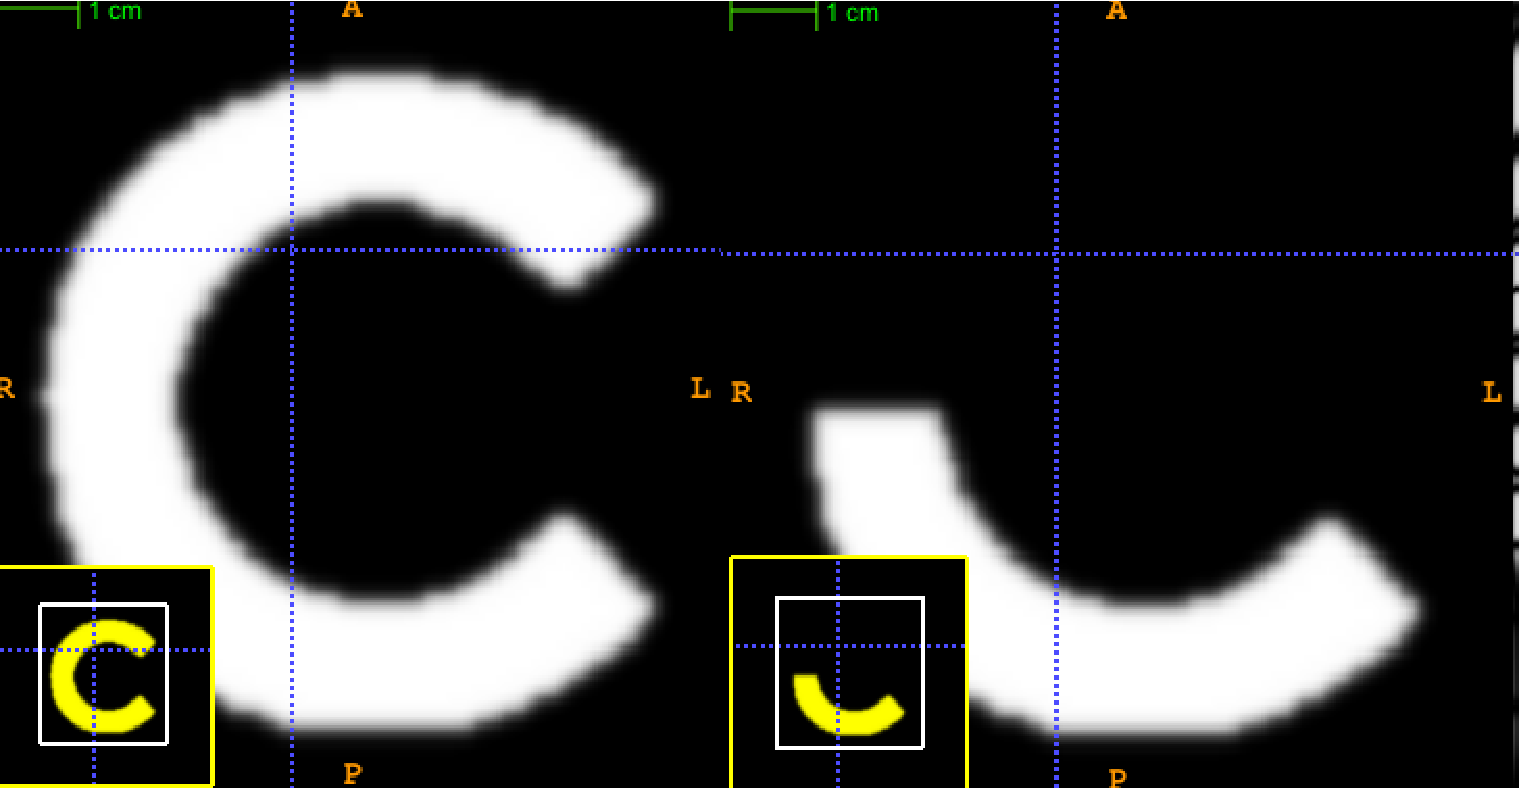
\includegraphics[height=1.1in]{figs/c_chalf.pdf}
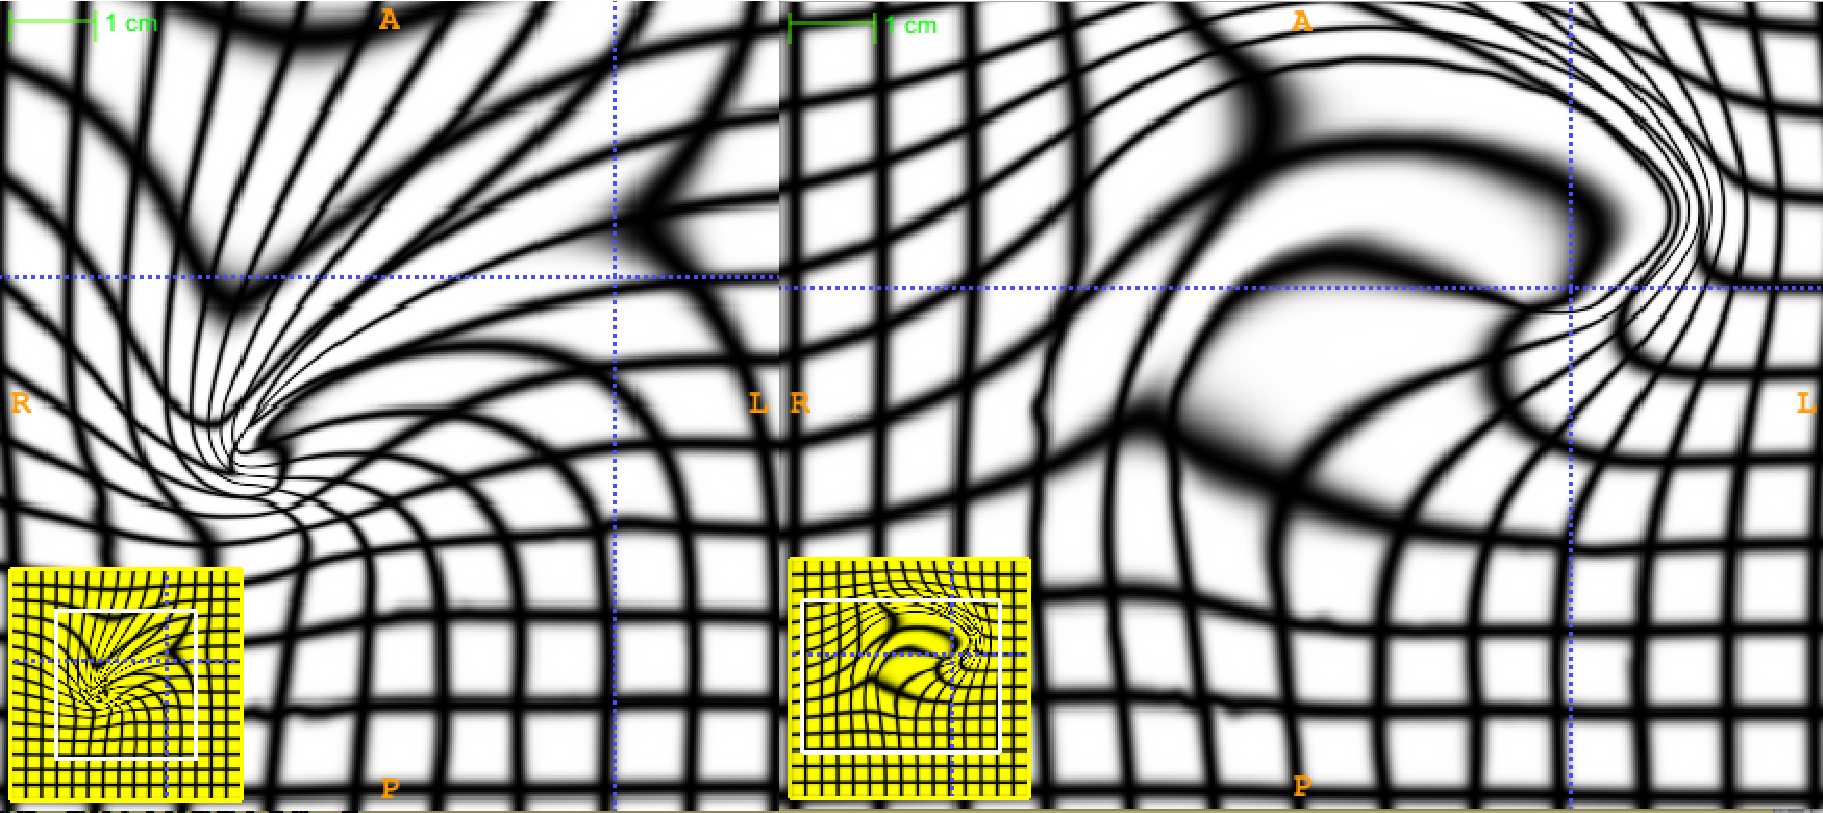
\includegraphics[height=1.1in]{figs/c_half_c_grids.pdf}
\end{tabular}
\caption{\baselineskip 12pt \small An ITK diffeomorphic mapping of the
  type $I \leftrightsquigarrow J $.  The 
``C'' and 1/2 ``C'' example illustrate the large deformations that may
be achieved with time varying velocity fields.  In this case, the moving (deforming) image is
the 1/2 ``C''.  The right panels illustrate the deformed grid for the
transformation of the ``C'' to 1/2 ``C'' (middle right) and its
inverse mapping (far right) which takes the 1/2 ``C'' to the reference
space.  The unit time interval is discretized into 15 segments in
order to compute this mapping.  15*5 integration steps were used in
the Runge-Kutta {\em ode} integration over the velocity field.  A two
core MacBook Air computed this registration in 110 seconds.  The images
each were of size $150 \times 150$.}
\label{fig:chalf}
\end{center}
\end{figure}

Beg proposed the Large Deformation Diffeomorphic Metric Mapping
(LDDMM) algorithm \cite{Miller2005} which minimizes the sum of squared differences
criterion between two images.  LDDMM parameterizes a
diffeomorphism through a time varying velocity field that is
integrated through an {\em ode}.  In \tk, we implement an alternative
to LDDMM that also uses a time varying field and an {\em ode} but minimizes
the following objective function:
\begin{align}
\myE(\v) = M(I,J,\myphi_{1,0})
+  w \int_{0}^{1} \| \opL v_t\|^2 \dd t \;.
\label{eq:lddmm}
\end{align}
This is an instance of equation~\ref{eq:gen} where $w$ is a scalar
weight and $\myphi_{1,0}$ is a standard integration of the
time-varying velocity field $v_t$ which is regularized by linear
operator $\opL$.  \tk uses Gaussian smoothing which is the Green's
kernel for generalized Tikhonov regularization \cite{Nielsen1997}.
This objective is readily optimized using an approach that is similar
to that proposed by Beg.  Generalization of the LDDMM gradient 
for other metrics basically follows \cite{hermosillo} with a few
adjustments to accomodate diffeomorphic mapping.
Figure~\ref{fig:chalf} shows an ITK result on a standard example for large
deformation registration.  We will evaluate this diffeomorphic
mapping, along with parameter estimation, in the following section.


\begin{comment}
{
Following \cite{hermosillo}, we
generalize the metric gradient such that correlation or mutual
information may be used.  
The \tk framework also has a novel minimization scheme that is based on fourth-order
Runge-Kutta integration and a new approach to enforcing the geodesic
condition that should be satisfied by $v_t$.  I.e. we minimize $D v /
dt $ where $D$ is the covariant derivative of the velocity
field.  $D v / dt = 0$ is a necessary condition for a geodesic;  Beg
reparameterizes the velocity field to be constant which is also a
necessary condition.  The advantage of our approach is that we can
easily incorporate the new criterion into the optimization by
smoothing the field, $v$, across time as well as space.  This is an
approximation of the covariant derivative that gets better as the
number of discretized time points increases.  
In this gradient-based optimization, the time-varying velocity fields are discretized into $N$ time points $(v_{t_i} )_{0 \leq i \leq N-1}$. For each time point $i$, the steepest descent scheme in the Sobolev space is applied:
\begin{eqnarray}
\u_{t_i} = \frac{\partial M(I_t,J_t,v)}{\partial J_t}\frac{\partial
  J(\phi_t)}{\partial \phi_t} \mathcal{J}
\; , 
\end{eqnarray}
where $\mathcal{J}$ is the Jacobian term as in the LDDMM gradient and
$I_t$ and $J_t$ represent $I$ and $J$ as they deform along the
geodesic defined by $v$.   We then use the following gradient update scheme,
\begin{eqnarray}
[ \v_1 \cdots \v_n ]\leftarrow G_\sigma \star (   [ \v_1 \cdots \v_n ]
+ \lambda  [ \u_1 \cdots \u_n ]   ) , \notag 
\end{eqnarray}
where $G_\sigma$ is a Gaussian operating across space and time, $[ \v_1 \cdots \v_n ]$ represents the discretized velocity field
(with $n$ discrete units)
and $[ \u_1 \cdots \u_n ]$ are the updates to the velocity field.
Note that if the smoothing $\sigma$ in the time domain is zero, this
approach defaults to a nearly standard LDDMM with the exception of our
higher-order integration procedure (fourth order Runge-Kutta).  The
derivation of the sum of squared differences gradient has been detailed in numerous other
publications. 
}
\end{comment}


\section{Evaluation}
We first investigate the ability of our automated parameter estimation
to facilitate parameter tuning across metrics.  We then compare \tk
with an open-source ITK$^3$ registration application.
In the future, the latest evaluation numbers will be available at:~\textcolor{blue}{
\href{https://github.com/stnava/ITKv4Documentation/tree/wbir2012}{ITKv4 latest
  evaluation results}}.
% \url{github.com/stnava/ITKv4Documentation}.
\subsection{Parameter estimation across metrics}
\tk provides similarity metrics that may be applied for both
deformable and affine registration.  In a previous section, we
provided a parameter estimation strategy that is applicable to both
deformable and affine transformations with arbitrary metrics.  Denote
images $I$, $J$, $K$, where the latter two are ``moving'' images, and
$K$ is an intensity-inverted version of $J$.
We then evaluate the following schema,
\begin{eqnarray}
I \approx \leftrightsquigarrow  \rightarrow J,~~~~~~~
I \approx_\text{cc} \leftrightsquigarrow  \rightarrow  K,~~~~~~~  
I \approx_\text{mi} \leftrightsquigarrow  \rightarrow  K   \notag 
\end{eqnarray}
where, for each schematic, we use the corresponding metric for both
affine and diffeomorphic mapping.  Furthermore, we keep the same
parameters for each registration by exploiting parameter scale
estimators.  Figure~\ref{fig:result} shows the candidate images for
this test. 

As shown in figure~\ref{fig:result}, very similar results are achieved
for each schematic without additional parameter tuning.  To determine
this quantitatively, we perform registration for each schematic and
then compare the Dice overlap of a ground-truth three-tissue
segmentation.  For each result, we have the Dice overlap of dark
tissue (cerebrospinal fluid, CSF), medium intensity tissue (gray
matter) and bright tissue (white matter).  For the mean squares
metric, we have: 0.588, 0.816 and 0.90; for CC, we have: 0.624, 0.786,
0.882; for MI, we have: 0.645, 0.779, 0.858.  Mutual information does
best for the CSF while mean squares does best for other tissues.  CC
performs in the mid-range for all classes of tissue.  Thus, a single
set of tuned parameters provides a reasonable result for an affine
plus diffeomorphic mapping across three different metrics.  While
improvement might be gained by further tuning for each metric, this
result shows that our parameter estimation method achieves the goal of
reducing user burden.
\begin{figure}[t]
\begin{center}
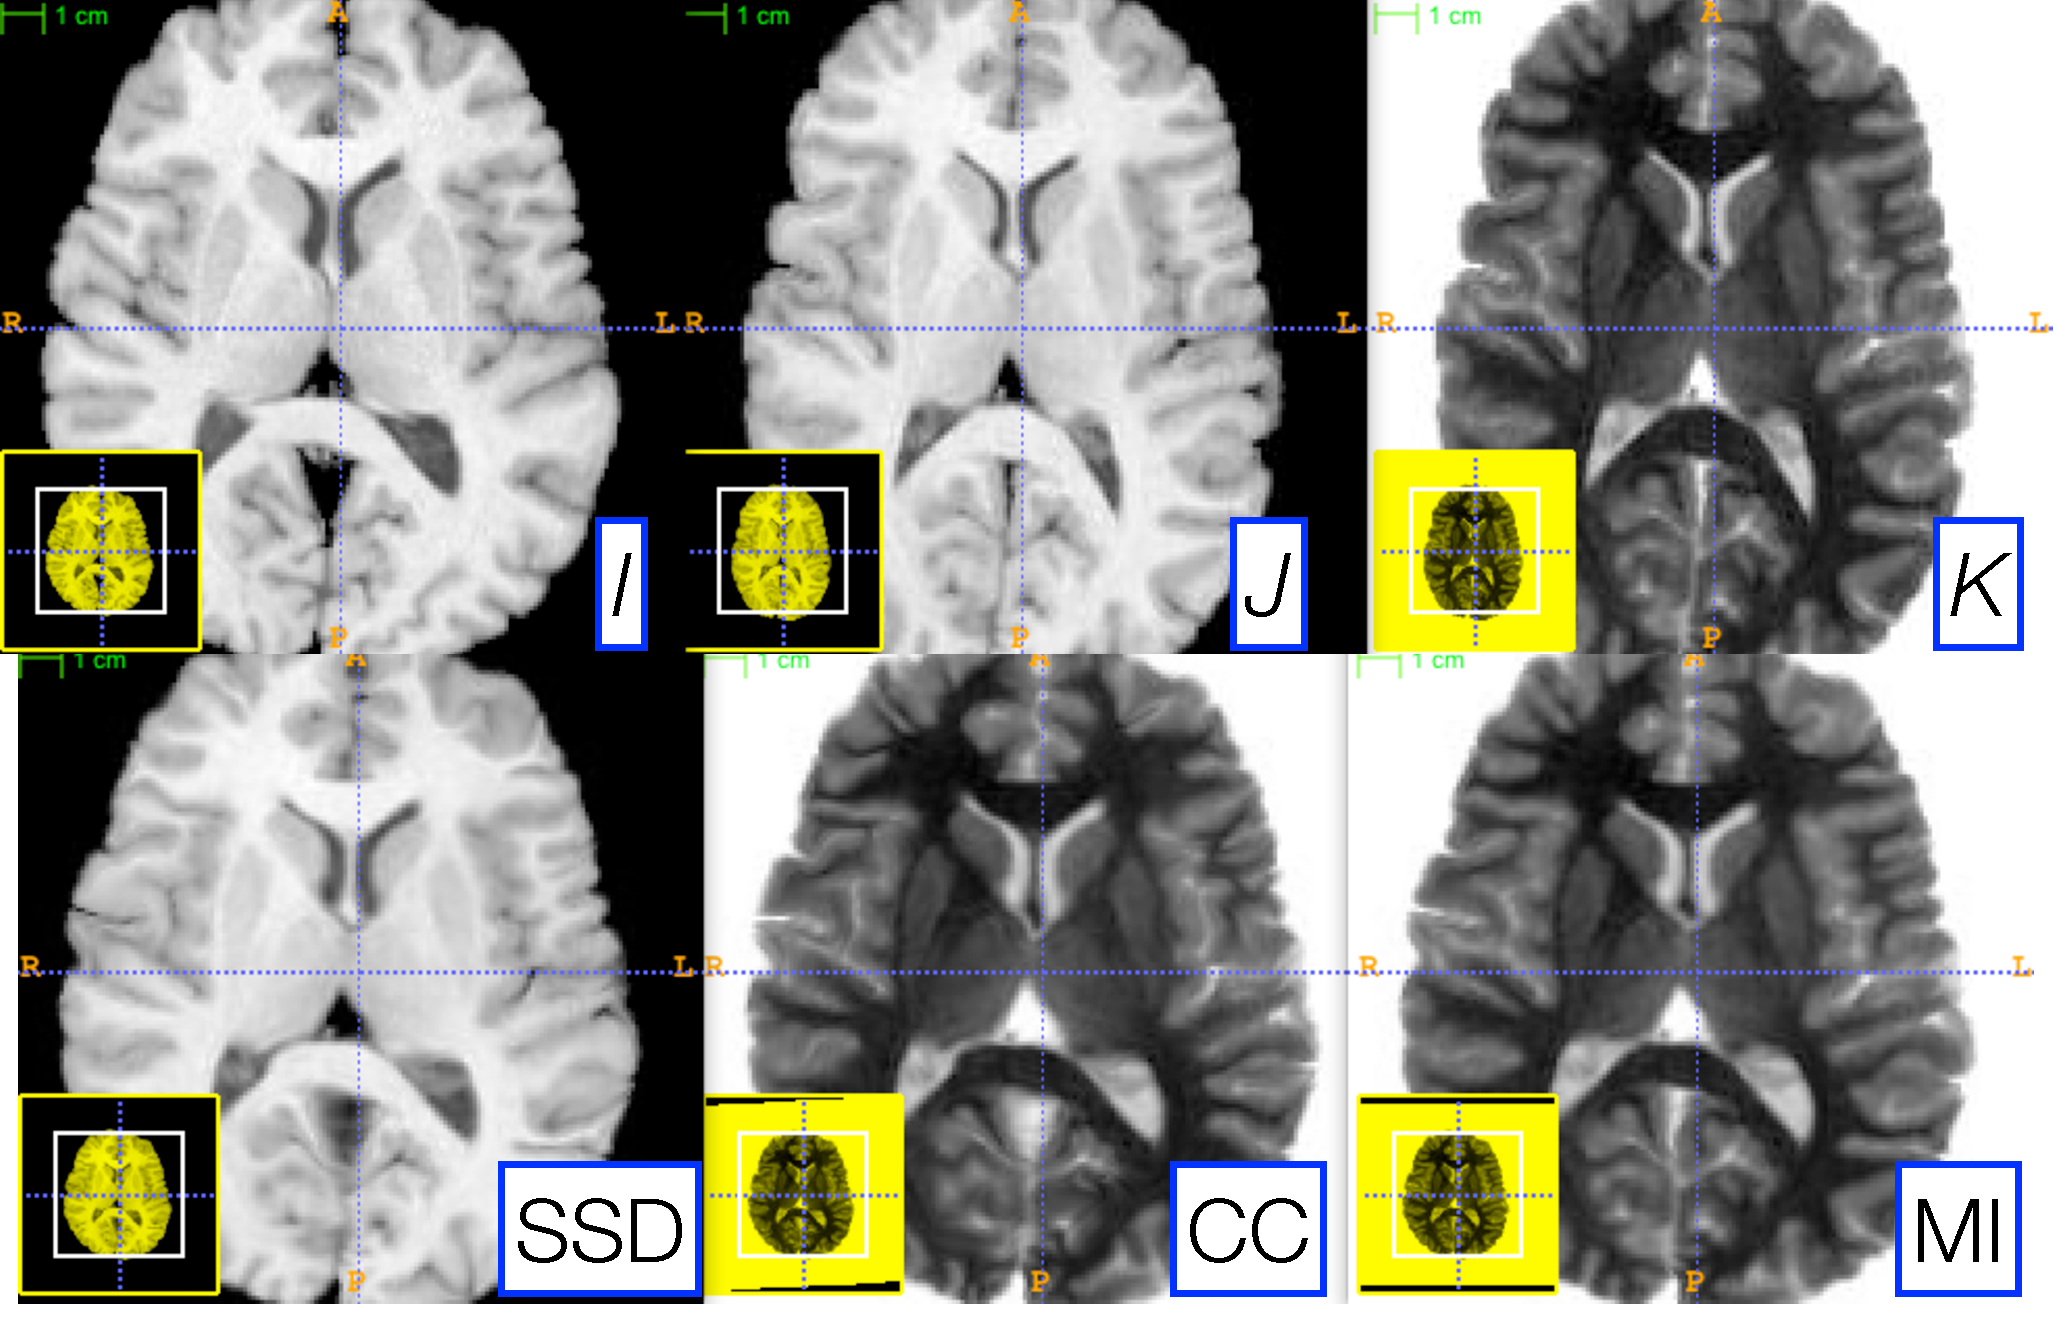
\includegraphics[width=3.5in]{figs/three.pdf}
\caption{\baselineskip 12pt \small Three references images, $I$
(left), $J$ (middle top), and $K$ (right top), are used to illustrate
the robustness of our parameter scale estimation for setting
consistent parameters across both metrics and transform types.  $K$ is
the negation of $J$ and is used to test the correlation and mutual
information registrations.  We optimized, by hand, the step-length
parameters for one metric (the sum of squared differences) for both the affine
and deformable case.  Thus, two parameters had to be optimized.  We
then applied these same parameters to register $I$ and $K$ via both
correlation and mutual information.  The resulting registrations
(bottom row) were all of similar quality.  Further, the same metric is
used for both affine and diffeomorphic mapping by exploiting the
general optimization process given in equation~\ref{eq:gen}.}
\label{fig:result}
\end{center}
\end{figure}


\begin{comment}{
Consider a velocity field that provides a geodesic (or shortest
distance) mapping between a pair of images, i.e. a registration of the
type $J  \leftrightsquigarrow \approx I$.  Because LDDMM does not
measure the change of the velocity field {\em over time}, the velocity
fields in this figure will have a measure of length that appears to be
equally ``geodesic.''  However, the velocity field at right, though of
constant arc length, will not minimize geodesic curvature.  Thus, we
augment the standard LDDMM measure of spatial regularity with a
measure of the change in velocity over time, $D v/ dt$, which
represents the covariant derivative of the velocity field.  Our
revised metric and the LDDMM metric will be equivalent if the velocity
field describes a true geodesic.
\begin{figure}[t]
\begin{center}
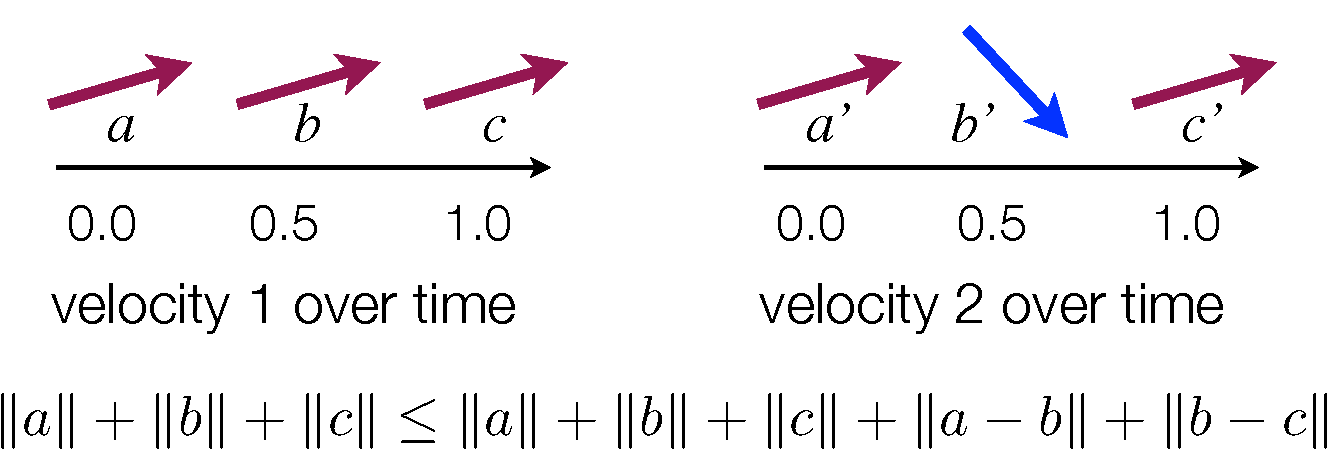
\includegraphics[width=4.5in]{figs/lddmm_comment.pdf}
\caption{\baselineskip 12pt \small Standard LDDMM minimizes a measure
  that integrates the velocity field's spatial
  regularity over time.  In \tk, we explore a novel extension to LDDMM
  that directly penalizes temporal discontinuities in the velocity field.  This \tk extension
  will prefer the solution at figure left over the solution at figure
  right.  On the other hand, if LDDMM is initialized with a velocity field that minimizes the
similarity metric---but is not a geodesic---LDDMM will not be able to emerge from that local
minimum.  This is because LDDMM does not directly penalize {\em
  acceleration} i.e. change in the velocity field.  Geodesic shooting
also resolves this shortcoming \cite{Beg2006}.}
\label{fig:geod}
\end{center}
\end{figure}
}\end{comment}


\subsection{Comparison against ITK$^3$}
We compare the \tk registration against an ITK$^3$ registration suite
BrainsFit (nitrc.org multimodereg).  
We present preliminary, encouraging evaluation results for this approach to
gradient descent with both affine and deformable registration in Figure~\ref{fig:eval}.
The dataset consists of ten elderly and demented subjects with manual labels of brain
parenchyma.  Of importance is that the ventricles are not included in
the parenchyma.  Large deformation is required to match ventricles
and, as such, this evaluation provides some insight into the benefit
of the new \tk diffeomorphic matching.
\begin{figure}[t]
\begin{center}
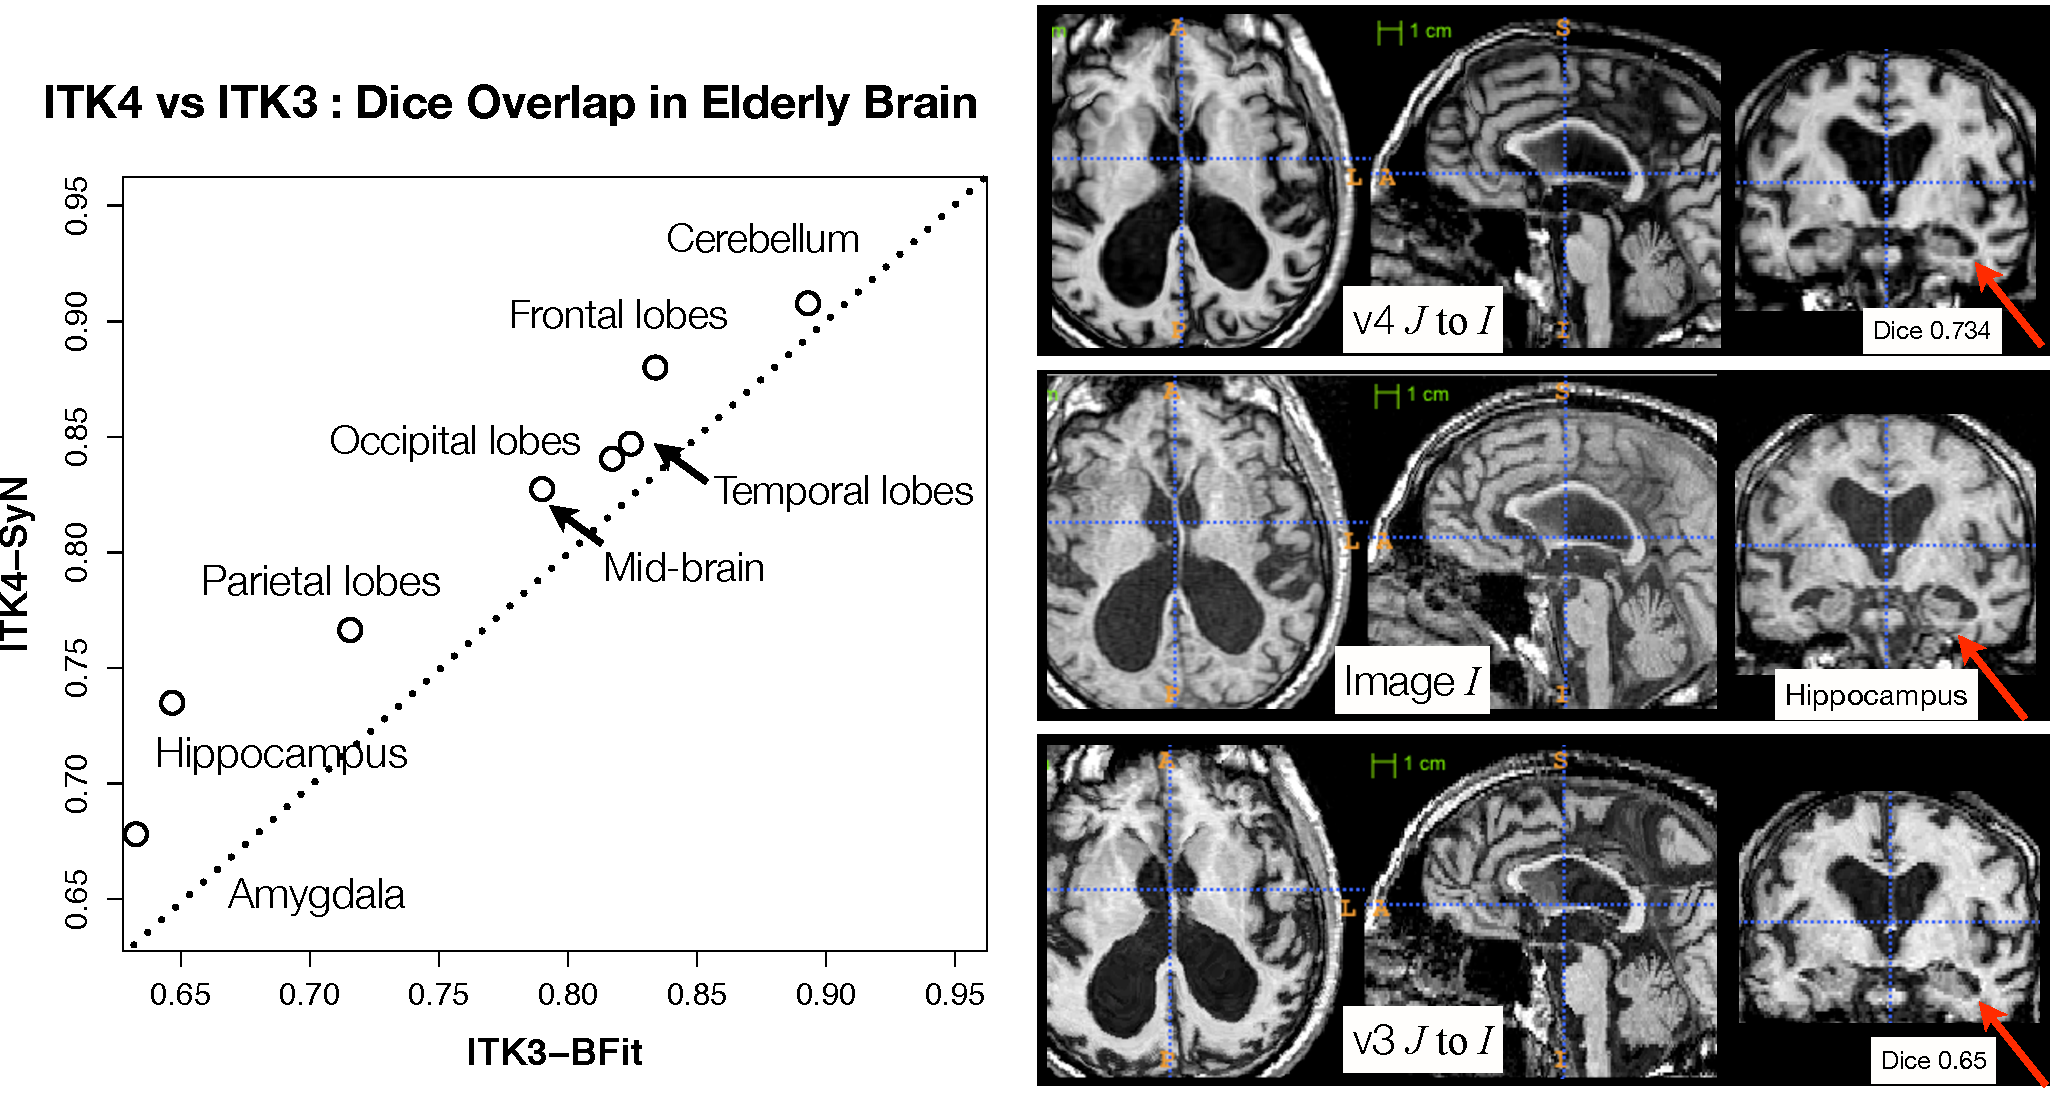
\includegraphics[width=4.5in]{figs/eval.pdf}
\caption{We compare an ITKv4 composite schema as $I
~\approx_\text{cc}  \leftrightsquigarrow \approx_\text{mi}  \rightarrow
J_i $ for mapping a set of $\{ J_i \}$ images
to a template $I$ to a v3 schema:  $I
~\approx_\text{mi} \rightsquigarrow_b    \approx_\text{mi}  \rightarrow
J_i $.  We use this schematic in a registration-based
segmentation of multiple brain structures in an elderly population as a benchmark
for algorithm performance, similar to \cite{Klein2010}.  Example
large-deformation results from the dataset are at right.  The largest
improvement in performance is within hippocampus, where a 13\%
improvement in v4 is gained.  Overlap improvement from v3 to v4, quantified via
paired t-test, is significant.  The example pair of images will be
included in v4 for regression testing.}
\label{fig:eval}
\end{center}
\end{figure}


\section{Discussion and future work} 
ITK is a community built and maintained toolkit and is a public
resource for reproducible methods.  The updated \tk registration
framework provides a novel set of user-friendly parameter setting
tools and benchmark implementations of both standard and advanced
algorithms.  Robustness with respect to parameter settings has long
been a goal of image registration and \tk takes valuable steps toward
the direction of automated parameter selection.  By the time of the
workshop, we intend to have a more extensive series of benchmark performance studies
completed on standard datasets and hope that presentation of this work
will provide a valuable foundation for future work.  The number of
possible applications exceeds what can possibly be evaluated via the
ITK core.  Community involvement is needed in order to increase the
number of possible registration applications and metric / transform /
optimizer / data combinations that have been evaluated.  At the same
time, documentation, usability and examples must be provided by the
development team in order to improve user involvement.  Future work
will enhance the depth and breadth of this documentation as well as
seek to optimize the current implementations for speed and memory.
With this effort, the user community will be capable of efficiently
implementing novel applications and even algorithms based on the \tk
framework.


\begin{comment}
{
\section{Deliverables}
\subsection{Usability}
\begin{description}
\item [Automate parameter scaling] base this on empirical statistics
  ``learning'' on a per registration problem basis.
\item [GetParameterSuggestion] metric and trasformation classes should
  recommend parameters from a developer-defined set.
\item [Multi-core implementations] multi threading of metric,
  regularization, parameter update, etc.  stephen indicates that the
  setparameters function may cause problems.   
\item [Unify the dense and sparse frameworks] metrics and
  transformations should be reusable across frameworks. 
\end{description}

\subsection{Data Types}
Transform vectors, curves and tensors with reorientation.

\subsection{Metrics}
\begin{description}
\item [metrics]  derivatives should be bi-directional.
\item [MI and NMI]  Shreyas --- MI and NMI multicore. 
\item [ATG Neighborhood Cross Correlation] our approximation to the
  NCC derivative.  
\item [PSE Metric] with arbitrary data type.  ObjectMetric ...
\item [Tractography/vector flow metric]  vector based.  distance transform?
\item [Multivariate metric] plug in metrics and weights and a
  ``combination'' strategy.  e.g. match 1-norm, 2-norm, etc before weighting. 
\end{description}

\subsection{Transformations}
\begin{description}
\item [BSpline]  Nick DMFFD and refactoring , bug fixing.  Usability
  and speed. 
\item [Composite transformation] need to get the composite derivatives
  right. 
\item [Deformation and rotation transform] have jeff implement.
  smooth rotation component internally (after update parameters).
\item [Velocity field] with fourth order integration.
\item [Reorientation transformation and derivative]  tensor and vector. 
\item [Rigid and deformable]  takes a mask that defines which parts
  are deformable and which are rigid.  the rigid parts are fixed by
  pre-computation.  the deformable parts are modified according to a
  registration strategy.  
\end{description}

\subsection{Regularization}
For instance, we should be able to compute a ``demons'' registration
without passing deformations to the filter.  We should pass
transformations (e.g. affine) and regularization (e.g. distance from
identity) in addition to the demons metric.  

\subsection{Longitudinal and serial registration}
Facilitate through transformations and regularization and unbiased design.
\begin{description}
\item [longitudinal] multiple images of the same subject over a longer time-scale.
\item [serial or time series] multiple images of the same subject or
  scene with high frequency sampling (samples that are dense in time).
\item [Longitudinal Image] Given a set of 3D images sampled
  longitudinally (see above), we package these $n$ images---along with
  $n$ rigid or affine transforms that map them to a common
  domain---into a standard itk image 
  interface.
\item [Serial image] this concept may already be supported.
\end{description}

\subsection{Algorithms}
\begin{description}
\item [SyN]  fully unbiased and lives as an algorithm (not
  multi-resolution) within ITK.   Multi-resolution SyN is a 2nd
  algorithm.  
\item [DMFFD] nick's style---greg's?
\item [Longitudinal Diffeomorphic Mapping] gang's version.
\item [vector versions of above]  ... with reorientation in
  transform.  also in optimization?
\end{description}


\section{The new framework}
Changes that we need to implement ASAP. 
\subsection{optimizers with regularization} We use the following
idea: any gradient based optimizer can be altered to perform the
following update scheme $ T_{i+1}=R(T_i + \lambda F(g))$ where $g$ is the
gradient and $\lambda$ is the update step.  The function $F$ is the
regularization on the gradient which will be dealt with by regularized
metrics.  So, this object should take a transform, an update to a 
transform and return the regularized transform $T_{i+1}$.  This requires a class of
optimizers that takes a regularization function as input \verb ->SetRegularizationFunction.  We will start with the gradient descent
optimizer.  Build a derived class that has a regularization function
and that overrides the update step to use that function.  It can be an
identity function for now.
\subsection{transform changes} The transforms should add a {\em thread-safe} function
called IncrementalUpdateToTransformParameters that takes a delta to
the parameters and updates the transform.  There will be an
implementation in the base class that just adds the parameters.  But
special transforms may want to override this function.  We also want a
function LocalJacobian which will default to the Jacobian computation
except in the cases where we override the function for the local,
dense transform types.
\subsection{deformation field transform} We need to resolve the
issues with the dense transform parameters.  I.e. map them
to an image efficiently or define a new local parameter type that is
based on the itkVector image.
\subsection{multivariate metric} Takes two ObjectToObjectMetrics as
input along with a weight function.  Defaults to uniform weighting
unless otherwise specified.  Weights are applied to the gradients of
the metric, not the metric itself.  
\subsection{multi-threading}  We need to be careful in making
decisions about all the above.  For instance, what is needed to make
the transforms thread-safe?   The regularizers?
\subsection{lightweight resampling}  Can we implement a lightweight
resample function that is local, thread-safe and samples an image in
such a way that code becomes more readable?  I.e. does the bounds
checking, reorientation, etc.  Relatedly, can the resample image
filter be rewritten with code reuse as an objective?
\subsection{multi-threaded metrics}  Gang wrote an initial
implementation.  We need to continue to work on this --- the demons
version needs to take a generic iterator type or allow different
iterators to be selected by the user.  

\subsection{the first new registration object}

SetImages 

SetRegistrationMachineryObjects --- what type of object is the
registration machinery?  really just a holder with reasonable defaults
for the stuff that needs to be set up.  Relies on get recommended
parameters and baohua's scale parameter setter to set up the defaults
for optimizer, metric etc.

SetOptimizer --- that will be in the machine but the optimizer might
have a regularization function which will have parameters.
Alternatively, we define regularized metrics that takes an
unregularized metric as input along with a regularizer and just
returns the regularized gradient---maybe a better idea!  A regularized
metric will project the gradient to the space in which it should
live.  

SetResolutions --- virtual domains along with scales?  kind of unclear 

SetVirtualDomain --- related to above 

RunRegistration --- given above, runs the registration.  Need a
convergence criterion.  

\section{Frobenius norm registration}
A three-dimensional problem with a derivative on $\x$, the spatial domain.
Let us assume that $\I \colon \Omega \in [0,1]^d \rightarrow
\mathbb{R}^d$ where $d$ defines the dimensionality. 
Homogeneous coordinates make this easier.
\begin{eqnarray}
T(\x) =\y = [A(\theta)] \phi(\x)= [A(\theta)] (\x+U(\x)) \\ \notag 
\J(T) = \R^T\J(\y)\R  \\ \notag 
\R =\text{R part of polar decomposition of }   \\ \notag
   [A(\theta)] (\Id+U_\x(\x))   \\ \notag
 \text{must compose affine with deformation gradient} \\ \notag
\text{in order that correctly reorients the data.}  \\ \notag
\| \I - \J (T) \|^2  \\ \notag 
\frac{\partial}{\partial \x} \| \I - \J (T) \|^2 \\ \notag
< \I - \J (T) , \frac{\partial}{\partial \x} (  \I - \J (T)  ) >  \\ \notag
\frac{\partial}{\partial \x} (  \I - \J (T)  ) =  \\ \notag
\frac{\partial}{\partial \x} \J (T)  =  \\ \notag
\text{ chain rule gets ugly ...}
\end{eqnarray}
}
\end{comment}
\bibliographystyle{splncs03}
\bibliography{./itk}
\end{document}
